\PassOptionsToPackage{unicode=true}{hyperref} % options for packages loaded elsewhere
\PassOptionsToPackage{hyphens}{url}
%
\documentclass[]{book}
\usepackage{lmodern}
\usepackage{amssymb,amsmath}
\usepackage{ifxetex,ifluatex}
\usepackage{fixltx2e} % provides \textsubscript
\ifnum 0\ifxetex 1\fi\ifluatex 1\fi=0 % if pdftex
  \usepackage[T1]{fontenc}
  \usepackage[utf8]{inputenc}
  \usepackage{textcomp} % provides euro and other symbols
\else % if luatex or xelatex
  \usepackage{unicode-math}
  \defaultfontfeatures{Ligatures=TeX,Scale=MatchLowercase}
\fi
% use upquote if available, for straight quotes in verbatim environments
\IfFileExists{upquote.sty}{\usepackage{upquote}}{}
% use microtype if available
\IfFileExists{microtype.sty}{%
\usepackage[]{microtype}
\UseMicrotypeSet[protrusion]{basicmath} % disable protrusion for tt fonts
}{}
\IfFileExists{parskip.sty}{%
\usepackage{parskip}
}{% else
\setlength{\parindent}{0pt}
\setlength{\parskip}{6pt plus 2pt minus 1pt}
}
\usepackage{hyperref}
\hypersetup{
            pdftitle={Outbreak Monitoring using ASMODEE: an example of automated data infrastructure},
            pdfauthor={Thibaut Jombart},
            pdfborder={0 0 0},
            breaklinks=true}
\urlstyle{same}  % don't use monospace font for urls
\usepackage{color}
\usepackage{fancyvrb}
\newcommand{\VerbBar}{|}
\newcommand{\VERB}{\Verb[commandchars=\\\{\}]}
\DefineVerbatimEnvironment{Highlighting}{Verbatim}{commandchars=\\\{\}}
% Add ',fontsize=\small' for more characters per line
\usepackage{framed}
\definecolor{shadecolor}{RGB}{248,248,248}
\newenvironment{Shaded}{\begin{snugshade}}{\end{snugshade}}
\newcommand{\AlertTok}[1]{\textcolor[rgb]{0.94,0.16,0.16}{#1}}
\newcommand{\AnnotationTok}[1]{\textcolor[rgb]{0.56,0.35,0.01}{\textbf{\textit{#1}}}}
\newcommand{\AttributeTok}[1]{\textcolor[rgb]{0.77,0.63,0.00}{#1}}
\newcommand{\BaseNTok}[1]{\textcolor[rgb]{0.00,0.00,0.81}{#1}}
\newcommand{\BuiltInTok}[1]{#1}
\newcommand{\CharTok}[1]{\textcolor[rgb]{0.31,0.60,0.02}{#1}}
\newcommand{\CommentTok}[1]{\textcolor[rgb]{0.56,0.35,0.01}{\textit{#1}}}
\newcommand{\CommentVarTok}[1]{\textcolor[rgb]{0.56,0.35,0.01}{\textbf{\textit{#1}}}}
\newcommand{\ConstantTok}[1]{\textcolor[rgb]{0.00,0.00,0.00}{#1}}
\newcommand{\ControlFlowTok}[1]{\textcolor[rgb]{0.13,0.29,0.53}{\textbf{#1}}}
\newcommand{\DataTypeTok}[1]{\textcolor[rgb]{0.13,0.29,0.53}{#1}}
\newcommand{\DecValTok}[1]{\textcolor[rgb]{0.00,0.00,0.81}{#1}}
\newcommand{\DocumentationTok}[1]{\textcolor[rgb]{0.56,0.35,0.01}{\textbf{\textit{#1}}}}
\newcommand{\ErrorTok}[1]{\textcolor[rgb]{0.64,0.00,0.00}{\textbf{#1}}}
\newcommand{\ExtensionTok}[1]{#1}
\newcommand{\FloatTok}[1]{\textcolor[rgb]{0.00,0.00,0.81}{#1}}
\newcommand{\FunctionTok}[1]{\textcolor[rgb]{0.00,0.00,0.00}{#1}}
\newcommand{\ImportTok}[1]{#1}
\newcommand{\InformationTok}[1]{\textcolor[rgb]{0.56,0.35,0.01}{\textbf{\textit{#1}}}}
\newcommand{\KeywordTok}[1]{\textcolor[rgb]{0.13,0.29,0.53}{\textbf{#1}}}
\newcommand{\NormalTok}[1]{#1}
\newcommand{\OperatorTok}[1]{\textcolor[rgb]{0.81,0.36,0.00}{\textbf{#1}}}
\newcommand{\OtherTok}[1]{\textcolor[rgb]{0.56,0.35,0.01}{#1}}
\newcommand{\PreprocessorTok}[1]{\textcolor[rgb]{0.56,0.35,0.01}{\textit{#1}}}
\newcommand{\RegionMarkerTok}[1]{#1}
\newcommand{\SpecialCharTok}[1]{\textcolor[rgb]{0.00,0.00,0.00}{#1}}
\newcommand{\SpecialStringTok}[1]{\textcolor[rgb]{0.31,0.60,0.02}{#1}}
\newcommand{\StringTok}[1]{\textcolor[rgb]{0.31,0.60,0.02}{#1}}
\newcommand{\VariableTok}[1]{\textcolor[rgb]{0.00,0.00,0.00}{#1}}
\newcommand{\VerbatimStringTok}[1]{\textcolor[rgb]{0.31,0.60,0.02}{#1}}
\newcommand{\WarningTok}[1]{\textcolor[rgb]{0.56,0.35,0.01}{\textbf{\textit{#1}}}}
\usepackage{longtable,booktabs}
% Fix footnotes in tables (requires footnote package)
\IfFileExists{footnote.sty}{\usepackage{footnote}\makesavenoteenv{longtable}}{}
\usepackage{graphicx,grffile}
\makeatletter
\def\maxwidth{\ifdim\Gin@nat@width>\linewidth\linewidth\else\Gin@nat@width\fi}
\def\maxheight{\ifdim\Gin@nat@height>\textheight\textheight\else\Gin@nat@height\fi}
\makeatother
% Scale images if necessary, so that they will not overflow the page
% margins by default, and it is still possible to overwrite the defaults
% using explicit options in \includegraphics[width, height, ...]{}
\setkeys{Gin}{width=\maxwidth,height=\maxheight,keepaspectratio}
\setlength{\emergencystretch}{3em}  % prevent overfull lines
\providecommand{\tightlist}{%
  \setlength{\itemsep}{0pt}\setlength{\parskip}{0pt}}
\setcounter{secnumdepth}{5}
% Redefines (sub)paragraphs to behave more like sections
\ifx\paragraph\undefined\else
\let\oldparagraph\paragraph
\renewcommand{\paragraph}[1]{\oldparagraph{#1}\mbox{}}
\fi
\ifx\subparagraph\undefined\else
\let\oldsubparagraph\subparagraph
\renewcommand{\subparagraph}[1]{\oldsubparagraph{#1}\mbox{}}
\fi

% set default figure placement to htbp
\makeatletter
\def\fps@figure{htbp}
\makeatother

\usepackage{booktabs}
\usepackage[]{natbib}
\bibliographystyle{apalike}

\title{Outbreak Monitoring using ASMODEE: an example of automated data infrastructure}
\author{Thibaut Jombart}
\date{2021-07-15}

\begin{document}
\maketitle

{
\setcounter{tocdepth}{1}
\tableofcontents
}
\hypertarget{preface}{%
\chapter*{Preface}\label{preface}}
\addcontentsline{toc}{chapter}{Preface}

\begin{center}\includegraphics[width=0.4\linewidth]{images/cover} \end{center}

The analysis pipeline described in this handbook is the result of the work of
many colleagues at the WHO and beyond. This includes, in alphabetic order:

\begin{itemize}
\item
  \emph{Code contributors in the COVID-19 analytics team}: Neale Batra, Finlay
  Campbell, Yuka Jinnai, Henry Laurenson-Schaffer
\item
  \emph{other code contributions}: Tim Taylor
\item
  \emph{feedback and inputs}: Brett Archer, Raquel Medialdea Carrera, Laura Guzman,
  Esther Hamblion, Orlagh Ingeborg, Zyleen Kassamali, Olivier le Polain,
  Katelijn Vandemaele
\item
  \emph{supervision}: Olivier le Polain
\end{itemize}

\hypertarget{intro}{%
\chapter{Introduction}\label{intro}}

Welcome to this short handbook describing an outbreak dynamics surveillance
system for COVID-19. This infrastructure was developed to provide weekly
assessments of risk levels for different countries in relation to the countries'
overall levels of infection, epidemic growth, and indications of trend
acceleration.

This infrastructure is written in \textbf{R}, and relies on the following key
components:

\begin{itemize}
\item
  \href{https://rmarkdown.rstudio.com/}{\emph{Rmarkdown}} (\texttt{.Rmd}) reports implementing
  the data gathering, preparation, analysis, and producing synthesis reports
\item
  the \href{https://www.reconverse.org/reportfactory/}{\emph{reportfactory}} providing the
  backbone of the infrastructure
\item
  a public \href{https://github.com/whocov/trend_analysis_public}{\emph{github}}
  repository used for hosting files, version control, and automation through
  \emph{github actions}
\end{itemize}

\hypertarget{what-does-this-infrastructure-do}{%
\section{What does this infrastructure do?}\label{what-does-this-infrastructure-do}}

This infrastructure provides an automated data pipeline that gathers publicly
available data on COVID-19 cases, deaths, tests, as well as on Variants of
Interest/Concerns (VoI / VoC) and vaccination by country, and provides a weekly
assessment of COVID-19 dynamics and levels of risks. The pipeline is implemented
as a \href{https://www.reconverse.org/reportfactory/}{reportfactory} which simplifies
the handling of dependencies, data and scripts, and enables the compilation of
analysis reports stored locally in dedicated, time-stamped folders.

A series of \texttt{Rmd} reports performs data gathering, various analysis, and produce
the following information products:

\begin{itemize}
\item
  png figures (\emph{pinplots} and \emph{tadpoles}) summarising the dynamics per WHO
  region, stored on github and visible on the
  \href{https://github.com/whocov/trend_analysis_public}{README.md} page (i.e.~landing
  page of the repository)
\item
  \texttt{rds} files containing the results for each WHO region, also stored on github,
  which can then be used for further investigation or for interactive dashboards
  (e.g.~shiny apps); some of these analyses are computer-intensive and would not
  be readily available on dashboards otherwise
\item
  automated emails to a specific list of recipients providing a detailed report
  of countries classified into epidemiological risk levels based on incidence,
  growth and trend changes; this latter part is not stored on github
\end{itemize}

\hypertarget{content-of-this-handbook}{%
\section{Content of this handbook}\label{content-of-this-handbook}}

This handbook is organised into the following chapters:

\begin{itemize}
\item
  \textbf{Chapter \ref{getting-started} - \protect\hyperlink{getting-started}{Getting started}}:
  instructions to run the infrastructure locally
\item
  \textbf{Chapter \ref{reports} - \protect\hyperlink{reports}{Reports overview}}: outline of the
  \texttt{Rmd} reports and how they interact
\item
  \textbf{Chapter \ref{asmodee} - \protect\hyperlink{asmodee}{Implementing ASMODEE}}: methodological
  and practical considerations for implementing ASMODEE, a new method for trend
  change detection
\item
  \textbf{Chapter \ref{automation} - \protect\hyperlink{automation}{Automation}}: details on how
  analyses are automated using github actions
\end{itemize}

\hypertarget{disclaimer}{%
\section{Disclaimer}\label{disclaimer}}

This repository contains work in progress. It implements an automated data pipeline for country-level surveillance of COVID-19 dynamics using publicly available data. Its content should not be used for publications without explicit agreement from the authors. The accuracy of the estimates provided in these analyses is contingent on data quality and availability. Results presented here do not represent the official view of the WHO, its staff or consultants. Caution must be taken when interpreting all data presented, and differences between information products published by WHO, national public health authorities, and other sources using different inclusion criteria and different data cut-off times are to be expected. While steps are taken to ensure accuracy and reliability, all data are subject to continuous verification and change. All counts are subject to variations in case detection, definitions, laboratory testing, vaccination strategy, and reporting strategies. See \url{https://covid19.who.int/info/} for further background and other important considerations surrounding the source data. The designations employed and the presentation of these materials do not imply the expression of any opinion whatsoever on the part of WHO concerning the legal status of any country, territory or area or of its authorities, or concerning the delimitation of its frontiers or boundaries. We seek to provide results for countries in all WHO regions (see inclusion criteria below). For technical reasons (missing data, low incidence, model not successfully fitting to the data), results may not be available for some countries. Where this happens, the list of missing countries is indicated in the relevant sections.

\hypertarget{licensing}{%
\section{Licensing}\label{licensing}}

This handbook is distributed under the creative-common attribution license
(CC-BY). See \href{https://creativecommons.org/licenses/by/2.0/}{this page} for more
information on the license.

Copyright holder: Thibaut Jombart, 2021

\hypertarget{getting-started}{%
\chapter{Getting started}\label{getting-started}}

In this chapter, we provide an overview of the infrastructure and of how the
data pipelines work. After outlining the main folders and files and their
respective roles, we provide installation guidelines and tips for using it
locally (i.e.~on your computer).

\hypertarget{overview-of-the-infrastructure}{%
\section{Overview of the infrastructure}\label{overview-of-the-infrastructure}}

The infrastructure implements data pipelines that download national COVID-19
data from online sources, performs some analyses, classify countries by
\textbf{epidemiological level of risk} (\textbf{ELR}) and produce synthesis reports which
can be emailed to a pre-defined list of recipients. It is summarised in figure
\ref{fig:overview}. The infrastructure itself is a
\href{https://www.reconverse.org/reportfactory/}{\emph{reportfactory}}, which provides a
structure for storing data, auxiliary scripts, reports sources and their
outputs. Its key components include:

\begin{itemize}
\tightlist
\item
  a set of \textbf{Rmarkdown reports} detailed in \textbf{chapter \ref{reports}}
\item
  a set of \textbf{github actions} implementing automated tasks on github servers, and
  detailed in \textbf{chapter \ref{automation}}
\end{itemize}

\begin{figure}

{\centering 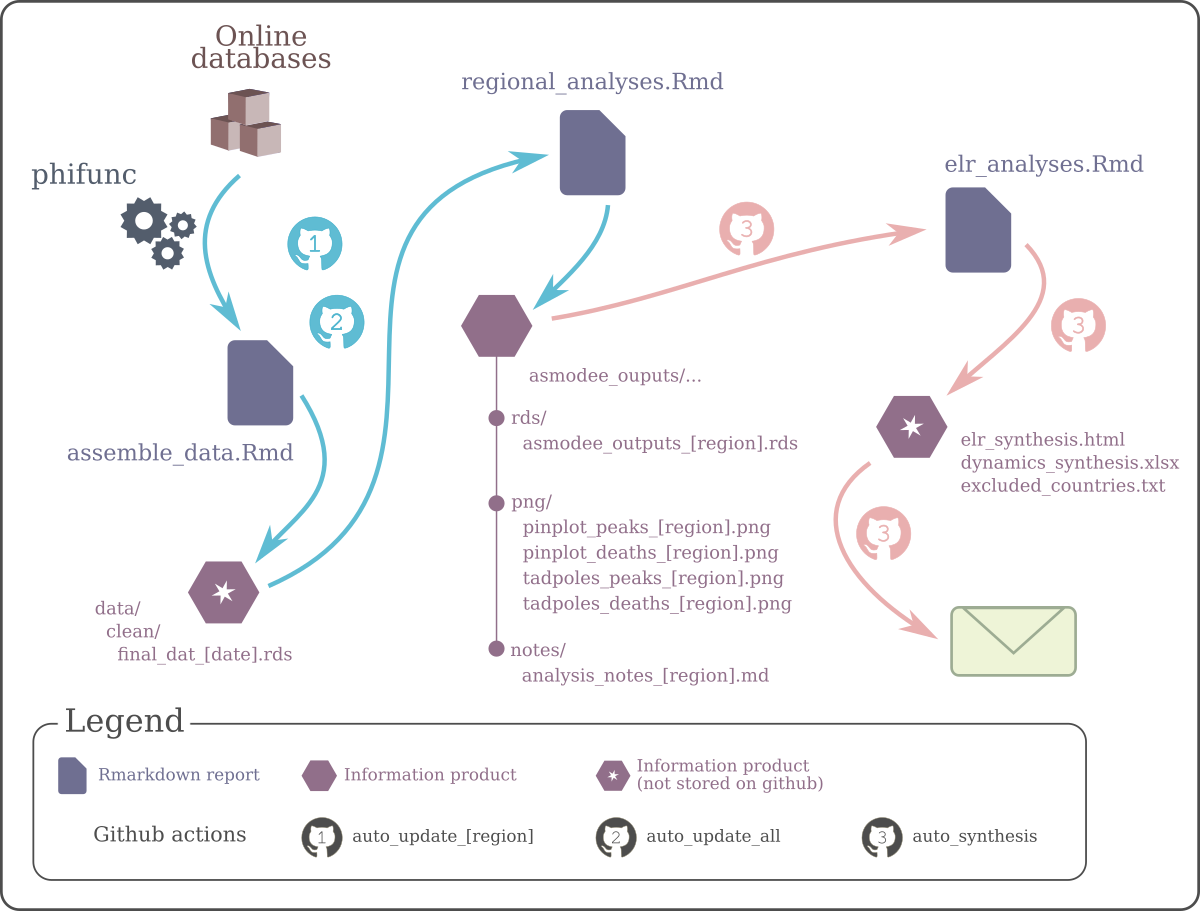
\includegraphics{images/reports_structure} 

}

\caption{Overview of the infrastructure. This diagram represents the flow of information processed by the data pipelines. Data are gathered from the net by the WHO-private package *phifunc*, and processed by a series of *Rmd* reports. Some of the information products generated, indicated by a star, are not stored on github in order to reduce the size of the repository. Upon compilation, all reports outputs are stored in an /outputs/ folder (not shown on the diagram). The automated email (last step) can only be sent by github actions, as it requires SMTP credentials only stored as github secrets.}\label{fig:overview}
\end{figure}

\hypertarget{main-folders-and-files}{%
\section{Main folders and files}\label{main-folders-and-files}}

The main components are:

\begin{itemize}
\item
  \textbf{data/}: a folder where raw and clean data are stored; the content of this
  folder is not stored on github to minimize the size of the git archive
\item
  \textbf{report\_sources/}: a folder containing the sources of the \texttt{Rmd} reports doing
  the data gathering and cleaning, and all analyses; see the \protect\hyperlink{reports}{reports}
  chapter for more information
\item
  \textbf{scripts/}: a folder containing \texttt{R} scripts used in the various reports; this
  includes small helper functions to load the latest versions of the data, help
  with bits of analysis, and code for installing packages not on CRAN, which
  cannot be handled automatically by \texttt{reportfactory::install\_deps()}
\item
  \textbf{outputs/}: a folder containing all compiled reports and associated outputs,
  in timestamped folders; this content is automatically generated when using
  \texttt{reportfactory::compile\_reports()}, and is only stored locally (i.e.~on your
  machine), and not on github (to keep the git archive to a minimal size)
\item
  \textbf{css/}: a folder containing styling for the reports
\item
  \textbf{asmodee\_outputs/}: a folder containing outputs of the main analysis, shared on
  github; this includes images (pinplots and tadpoles), \textbf{R} objects (\texttt{rds}
  files) containing re-usable analysis results (e.g.~for inclusion in websites
  or dashboards), and analysis notes (indicating excluded countries, and reasons
  for their exclusions)
\item
  \textbf{docs/}: a folder containing the sources and compiled versions of this
  handbook
\end{itemize}

Other useful files and folders to know of include:

\begin{itemize}
\item
  \textbf{README.Rmd}: the source of the \texttt{README.md} file, which is displayed on the
  landing package of the \href{https://github.com/whocov/trend_analysis_public}{github project},
  and shows the latest tadpoles figures by WHO region and also provides links to
  the corresponding \texttt{rds} files
\item
  \textbf{run\_factory.R}: the main R script for updating data, and running analysis
  reports for every WHO regions; also used by github actions
\item
  \textbf{run\_synthesis.R}: an R script used in github actions to generate a synthesis
  report for all countries, including a classification into levels of risk based
  on incidence, growth and trend acceleration, and for sending an email to a list of
  recipients with these documents attached
\item
  \textbf{.github/workflows/}: a (hidden) folder storing the files used to define the
  github actions; see the \protect\hyperlink{automation}{automation} chapter for more information
\item
  \textbf{factory\_config}: a simple text file containing some information about the
  name of key directories of the factory; normally will not need editing, unless
  you rename the folder containing the factory (see \ref{downloading})
\end{itemize}

\hypertarget{installing-the-infrastructure}{%
\section{Installing the infrastructure}\label{installing-the-infrastructure}}

The infrastructure can be installed locally by downloading the repository from
github and installing dependencies. To run the full pipeline, the user will need
an authentication token used to install the private (i.e.~not publicly
available) WHO package \texttt{phifunc}, which is used for collating data.

\hypertarget{downloading}{%
\subsection{Downloading the repository}\label{downloading}}

You can download the repository from the \textbf{code} tab on the
\href{https://github.com/whocov/trend_analysis_public}{github page}
as illustrated in the figure \ref{fig:download}.

\begin{figure}

{\centering \includegraphics[width=1\linewidth]{images/download} 

}

\caption{Downloading or cloning the repository. The repository containing the data infrastructure can be downloaded as a zip archive or cloned using github.}\label{fig:download}
\end{figure}

We recommend using \emph{SSH} to clone the repository. For more information on
setting up an SSH access to github, see this
\href{https://docs.github.com/en/github/authenticating-to-github/connecting-to-github-with-ssh}{webpage}.

Once you are set up to access github using SSH, you can clone the repository
using GIT from the command line in your favourite terminal, by typing:

\begin{Shaded}
\begin{Highlighting}[]
\FunctionTok{git}\NormalTok{ clone git@github.com:whocov/trend_analysis_public.git}
\end{Highlighting}
\end{Shaded}

The advantage of cloning the repository rather than merely downloading a zip
archive is that you will be able to update the infrastructure automatically
using \texttt{git\ pull}.

By default, your local copy of the repository will be called
\emph{trend\_analysis\_public}. It is possible to change this name, but you will need
to update the name of the factory in the \textbf{factory\_config} file. From now on,
we will refer to this folder as \textbf{root folder}.

\hypertarget{getting-the-phifunc-authentication-token}{%
\subsection{Getting the phifunc authentication token}\label{getting-the-phifunc-authentication-token}}

The tool we use to collate COVID-19 data is a package called \texttt{phifunc} developed
at WHO. Because this package internally uses some non-public data API, it is
currently not shared publicly, and an \textbf{authentication token} is needed to be
able to install it in \textbf{R}. This token is a kind of \emph{password}, stored in a
file called \texttt{phifunc\_token} in the root folder.

The easiest way to add this file is ask for it from someone in the COVID-19
analytics team, and add this file to the root of the project. Make sure you do
not alter or rename it. Once \texttt{phifunc\_token} is present in your infrastructure,
the scripts installing dependencies will detect it automatically when run, and
you will be able to run all analyses locally.

\hypertarget{installing-dependencies}{%
\subsection{Installing dependencies}\label{installing-dependencies}}

To install the dependencies, open the reportfactory by double-clicking on
\texttt{open.Rproj}, or otherwise starting an R session in the \textbf{root} folder
(\emph{trend\_analysis\_public} by default), and copy-paste the following commands:

\begin{Shaded}
\begin{Highlighting}[]

\CommentTok{# install basic packages}
\NormalTok{pkg <-}\StringTok{ }\KeywordTok{c}\NormalTok{(}\StringTok{"remotes"}\NormalTok{, }\StringTok{"reportfactory"}\NormalTok{)}
\KeywordTok{install.packages}\NormalTok{(pkg)}

\CommentTok{# install deps for the factory}
\NormalTok{reportfactory}\OperatorTok{::}\KeywordTok{install_deps}\NormalTok{()}
\KeywordTok{source}\NormalTok{(here}\OperatorTok{::}\KeywordTok{here}\NormalTok{(}\StringTok{"scripts"}\NormalTok{, }\StringTok{"remote_packages.R"}\NormalTok{))}
\end{Highlighting}
\end{Shaded}

Note that the last operation will require the authentication token (file
\texttt{phifunc\_token}) for installing \emph{phifunc}. We will be working separately on a
similar infrastructure using data that are directly publicly available.

\hypertarget{running-the-infrastructure-locally}{%
\section{Running the infrastructure locally}\label{running-the-infrastructure-locally}}

The data infrastructure can run in two modes:

\begin{itemize}
\item
  \textbf{remotely}, through github actions; this happens at specific times but can also
  be triggered manually
\item
  \textbf{locally}, on your computer
\end{itemize}

Here, we outline the \emph{local} use. You will find more information about the
github actions in the \protect\hyperlink{automation}{automation} chapter.

\hypertarget{updating-all-analyses}{%
\subsection{Updating all analyses}\label{updating-all-analyses}}

The simplest way to update all analyses is run the script \texttt{run\_factory.R} (using
\texttt{source(run\_factory.R)}, or step-by-step by opening the file in Rstudio). This
will:

\begin{itemize}
\tightlist
\item
  download, assemble and pre-process the most recent data
\item
  run a separate report for each WHO region, storing timestamped output in the
  \texttt{outputs/} folder, as well as figures, notes, and \emph{rds} files in the
  \texttt{asmodee\_outputs} folder
\item
  update the \emph{README} file with the new analyses
\end{itemize}

\hypertarget{updating-the-data}{%
\subsection{Updating the data}\label{updating-the-data}}

The report \texttt{assemble\_data.Rmd} performs the data download, gathering and
preparation. To update the data, run the following command within the factory:

\begin{Shaded}
\begin{Highlighting}[]

\KeywordTok{library}\NormalTok{(reportfactory)}
\KeywordTok{compile_reports}\NormalTok{(}\DataTypeTok{report =} \StringTok{"assemble"}\NormalTok{)}
\end{Highlighting}
\end{Shaded}

\hypertarget{running-analyses-for-a-specific-region}{%
\subsection{Running analyses for a specific region}\label{running-analyses-for-a-specific-region}}

The report \texttt{regional\_analyses.Rmd} performs all analyses for a given WHO region,
including calculations of growth rates and trend change detection using
ASMODEE. The report automatically uses the latest version of the clean data (so
needs to be run after \texttt{assemble\_data.Rmd} if the data need updating). The
parameter \texttt{who\_region} determines which WHO region is analysed. Possible values
are: \texttt{AFRO}, \texttt{EMRO}, \texttt{EURO} (default), \texttt{PAHO}, \texttt{SEARO}, \texttt{WPRO}. To run the
report, type:

\begin{Shaded}
\begin{Highlighting}[]

\KeywordTok{library}\NormalTok{(reportfactory)}
\NormalTok{reg <-}\StringTok{ "EURO"} \CommentTok{# replace as appropriate}
\NormalTok{cores <-}\StringTok{ }\DecValTok{4}
\KeywordTok{compile_reports}\NormalTok{(}\DataTypeTok{report =} \StringTok{"regional_analyses"}\NormalTok{,}
                \DataTypeTok{params =} \KeywordTok{list}\NormalTok{(}\DataTypeTok{who_region =}\NormalTok{ reg, }\DataTypeTok{n_cores =}\NormalTok{ cores),}
                \DataTypeTok{subfolder =}\NormalTok{ reg)}
\end{Highlighting}
\end{Shaded}

where:

\begin{itemize}
\tightlist
\item
  \texttt{reg} is the letter code for the WHO region to use (in upper case)
\item
  \texttt{cores} is the number of cores to be used for the ASMODEE analyses, which
  support parallelisation
\item
  \texttt{subfolder} indicates the name of the folder in \texttt{outputs} where the
  timestamped results will be stored
\end{itemize}

\hypertarget{generating-the-synthesis-report}{%
\subsection{Generating the synthesis report}\label{generating-the-synthesis-report}}

The report \texttt{elr\_synthesis} collates the latest results for all WHO regions,
classifies countries by level of risk, and produces a synthesis html report,
alongside an .xlsx file \texttt{dynamics\_summary.xlsx} summarising results and a list
of excluded countries in the text file \texttt{excluded\_countries.txt}.

To compile this report, use:

\begin{Shaded}
\begin{Highlighting}[]

\KeywordTok{library}\NormalTok{(reportfactory)}
\KeywordTok{compile_reports}\NormalTok{(}\DataTypeTok{report =} \StringTok{"elr_synthesis"}\NormalTok{)}
\end{Highlighting}
\end{Shaded}

\hypertarget{reports}{%
\chapter{Overview of the reports}\label{reports}}

This chapter provides some additional informations about the different
\emph{Rmarkdown} reports. For details of data processing and analyses, we refer to
the respective documents, as we attempted to document all code in each
report. We recommend compiling the reports first and looking at the \emph{html}
outputs generated as a more user-friendly alternative to inspecting the source
code directly.

Reports can be \textbf{compiled} by two ways:

\begin{enumerate}
\def\labelenumi{\arabic{enumi}.}
\item
  using \texttt{reportfactory::compile\_reports(...)} where \texttt{...} is a character string
  matching the name(s) of the reports to be processed (regular expression
  accepted); outputs will be stored in time-stamped folders inside \emph{outputs/}
\item
  using the usual \texttt{rmarkdown::render(...)} where \texttt{...} is the path of the \texttt{Rmd}
  document to process; outputs will be stored inside \emph{report\_sources/}
\end{enumerate}

Some reports accept \textbf{parameters}, i.e.~variables set at compilation time which can
impact the results generated. This is typically used, for instance, to indicate
which WHO region the analyses are to be performed on, and is a more sustainable
alternative to handling separate reports for every region. For both compilation
methods the way to specify parameters to a report is the same; passing a list
called \texttt{param} when compiling documents. For instance:

\begin{Shaded}
\begin{Highlighting}[]
\KeywordTok{library}\NormalTok{(reportfactory)}
\KeywordTok{compile_reports}\NormalTok{(}\DataTypeTok{report =} \StringTok{"analyses"}\NormalTok{,}
                \DataTypeTok{params =} \KeywordTok{list}\NormalTok{(}\DataTypeTok{who_region =} \StringTok{"AFRO"}\NormalTok{)}
\end{Highlighting}
\end{Shaded}

will compile the analysis report \emph{regional\_analyses.Rmd} (only match for the
word \texttt{"analyses"}) for the AFRO region.

\textbf{Default values of parameters} are set in the YAML headers of the respective
reports.

\hypertarget{data-preparation-assemble_data.rmd}{%
\section{\texorpdfstring{Data preparation: \emph{assemble\_data.Rmd}}{Data preparation: assemble\_data.Rmd}}\label{data-preparation-assemble_data.rmd}}

This report downloads the data and pre-processes it to enable further analyses.

\hypertarget{inputs}{%
\subsection{Inputs}\label{inputs}}

The package \emph{phifunc} is used to download publicly-available, national COVID-19
data, and to do some of the pre-processing. Unfortunately, this package uses WHO
internal APIs for some of these tasks and cannot be made publicly available
without exposing these APIs, which would be a security breach. As a result, the
package can only be installed with an \textbf{authentication token}, which needs to be
stored in a file called \emph{phifunc\_token} at the root of the project folder.

\hypertarget{outputs}{%
\subsection{Outputs}\label{outputs}}

The main output of the report is a clean data file containing data for all
countries named \emph{final\_dat\_{[}date{]}.rds}, a copy of which will be stored in the
\emph{data/clean} folder. These files are ignored by \emph{git}, and will not be added to
the \emph{github} repository to reduce the size of the archive.

\hypertarget{parameters}{%
\subsection{Parameters}\label{parameters}}

The report accepts the following parameters:

\begin{itemize}
\tightlist
\item
  \texttt{import\_data}: a \texttt{logical} indicating if the data should be downloaded
  (\texttt{TRUE}, default), or if local copies of the last raw data downloaded should
  be used (\texttt{FALSE})
\end{itemize}

\hypertarget{example-compilation}{%
\subsection{Example compilation}\label{example-compilation}}

The following instructions will compile the report:

\begin{Shaded}
\begin{Highlighting}[]
\KeywordTok{library}\NormalTok{(reportfactory)}
\KeywordTok{compile_reports}\NormalTok{(}\DataTypeTok{report =} \StringTok{"assemble"}\NormalTok{)}
\end{Highlighting}
\end{Shaded}

\hypertarget{analyses-of-covid-19-dynamics-regional_analyses.rmd}{%
\section{\texorpdfstring{Analyses of COVID-19 dynamics: \emph{regional\_analyses.Rmd}}{Analyses of COVID-19 dynamics: regional\_analyses.Rmd}}\label{analyses-of-covid-19-dynamics-regional_analyses.rmd}}

This report uses the latest clean data to perform a range of analyses for a
specific WHO region. Analyses include estimation of the growth rate, detection
of trend changes using ASMODEE, and figures summarising the overall dynamics of
COVID-19 by country (pinplots and tadpoles).

\hypertarget{inputs-1}{%
\subsection{Inputs}\label{inputs-1}}

The latest data are automatically detected and loaded by the auxiliary function
\texttt{load\_final\_data()}, defined in \emph{scripts/data\_loaders.R}

\begin{figure}

{\centering \includegraphics{images/example_pinplot} 

}

\caption{Example of pinplot. This figure summarises the dynamics of COVID-19 at a national level, using three complementary metrics: the daily growth rate *r* (*x* axis), the currentl weekly incidence (*y* axis), and the number of net increases showing trend acceleration detected by ASMODEE (colors). Another variant of this figure uses weekly incidence of deaths per capita on the *y* axis. Countries to the right show faster epidemic growth, and countries near the top experience high levels of incidence. Countries displayed in red show signs of acceleration, so that they may move further to the right in the coming days. This figure was generated for EMRO on 11th July 2021.}\label{fig:pinplot}
\end{figure}

\hypertarget{outputs-1}{%
\subsection{Outputs}\label{outputs-1}}

The main output of the report is a \texttt{list} exported as a file named
\emph{asmodee\_outputs}{[}WHO region{]}\emph{{[}data{]}.rds} stored in \emph{/asmodee\_outputs/rds/}, and
containing the following elements:

\begin{itemize}
\tightlist
\item
  \texttt{\$summary}: summary of the ASMODEE results
\item
  \texttt{\$results}: outputs of ASMODEE
\item
  \texttt{\$plot\_overall\_deaths}: \emph{ggplot2} object of the overall dynamics plot using
  death per capita on the y-axis
\item
  \texttt{\$plot\_overall\_peaks}: \emph{ggplot2} object of the overall dynamics plot using
  incidence as percentage of historical peak on the y-axis
\item
  \texttt{\$df\_dynamics}: a \texttt{data.frame} containing all the required info to recreate
  either global dynamics plots
\item
  \texttt{\$elr\_extras}: a \texttt{data.frame} containing additional information for countries,
  including TPR and vaccination coverage
\item
  \texttt{\$timestamp}: the timestamp corresponding to the date of the dataset used in
  the analyses
\end{itemize}

Other outputs include:

\begin{itemize}
\item
  \textbf{pinplots} and \textbf{tadpoles} figures saved \emph{asmodee\_outputs/png/}; these
  figures summarise the COVID-19 dynamics according to the \emph{growth rate}, the
  current weekly \emph{incidence}, and the number of net accelerations identified by
  ASMODEE; pinplots show the current situation (see example in Figure
  \ref{fig:pinplot}, while tadpoles show the trajectories of countries over the
  last few days
\item
  \textbf{notes} listing countries what were excluded from the analyses alongside the
  reason for their exclusion, stored in a markdown file named \emph{analysis\_notes}{[}WHO
  region{]}\emph{{[}data{]}.md} stored in \emph{/asmodee\_outputs/notes/}
\end{itemize}

\hypertarget{parameters-1}{%
\subsection{Parameters}\label{parameters-1}}

The report accepts the following parameters:

\begin{itemize}
\item
  \texttt{who\_region}: the code of the WHO region used in the analyses; possible values
  are (keep the upper case): \texttt{AFRO}, \texttt{EMRO}, \texttt{EURO} (default), \texttt{PAHO}, \texttt{SEARO},
  \texttt{WPRO}
\item
  \texttt{n\_cores}: the number of cores/processors to be used for ASMODEE; as the
  method supports parallelisation, more cores usually mean faster analyses;
  defaults to 1 (no parallelisation)
\item
  \texttt{tadpole\_size}: the number of days to be considered when showing the
  trajectories of the countries on tadpoles plots; defaults to 7
\end{itemize}

\hypertarget{example-compilation-1}{%
\subsection{Example compilation}\label{example-compilation-1}}

The following instructions will compile the report for EMRO, using 12 cores for
the calculations; also note the use of \texttt{subfolder} which will ensure that
results are stored in a timestamped folder in \emph{outputs/EMRO/} (rather than in
\emph{outputs/}):

\begin{Shaded}
\begin{Highlighting}[]

\KeywordTok{library}\NormalTok{(reportfactory)}
\NormalTok{rmarkdown}\OperatorTok{::}\KeywordTok{render}\NormalTok{(}\StringTok{'regional_analyses'}\NormalTok{,}
                  \DataTypeTok{params =} \KeywordTok{list}\NormalTok{(}\DataTypeTok{n_cores =} \DecValTok{12}\NormalTok{, }\DataTypeTok{who_region =} \StringTok{"EMRO"}\NormalTok{),}
                  \DataTypeTok{subfolder =} \StringTok{"EMRO"}\NormalTok{)}
\end{Highlighting}
\end{Shaded}

The following loop will do the same but for every region:

\begin{Shaded}
\begin{Highlighting}[]

\KeywordTok{library}\NormalTok{(reportfactory)}
\NormalTok{regions <-}\StringTok{ }\KeywordTok{c}\NormalTok{(}\StringTok{"AFRO"}\NormalTok{, }\StringTok{"EMRO"}\NormalTok{, }\StringTok{"EURO"}\NormalTok{, }\StringTok{"PAHO"}\NormalTok{, }\StringTok{"SEARO"}\NormalTok{, }\StringTok{"WPRO"}\NormalTok{)}

\ControlFlowTok{for}\NormalTok{ (reg }\ControlFlowTok{in}\NormalTok{ regions) \{}
\NormalTok{rmarkdown}\OperatorTok{::}\KeywordTok{render}\NormalTok{(}\StringTok{'regional_analyses'}\NormalTok{,}
                  \DataTypeTok{params =} \KeywordTok{list}\NormalTok{(}\DataTypeTok{n_cores =} \DecValTok{12}\NormalTok{, }\DataTypeTok{who_region =}\NormalTok{ reg),}
                  \DataTypeTok{subfolder =}\NormalTok{ reg)}
\NormalTok{\}}
\end{Highlighting}
\end{Shaded}

\hypertarget{synthesis-elr_synthesis.rmd}{%
\section{\texorpdfstring{Synthesis: \emph{elr\_synthesis.Rmd}}{Synthesis: elr\_synthesis.Rmd}}\label{synthesis-elr_synthesis.rmd}}

This report compiles results of all WHO regions, defines ELR for the countries,
and stores the main results into an \emph{xlsx} file.

\hypertarget{inputs-2}{%
\subsection{Inputs}\label{inputs-2}}

The report compiles the latest results obtained for the different WHO regions
stored in \texttt{asmodee\_outputs/rds/}.

\hypertarget{outputs-2}{%
\subsection{Outputs}\label{outputs-2}}

Based on the metrics used in the pinplots, countries are assigned an ELR using
the algorithm summarised in figure \ref{fig:elr-algo}. The report provides
complementary informations including trend plots (ASMODEE results) for the
countries with \emph{Medium} risk or higher, and some additional information on
Testing Positivity Rates (TPR) and vaccination coverage.

\begin{figure}

{\centering \includegraphics[width=0.75\linewidth]{images/elr_algo} 

}

\caption{Algorithm to define Epi Level of Risk (**ELR**). This diagram summarises the algorithm used to define a risk level (*Low* / *Medium* / *High* / *Very High*) based on values of the daily growth rates, weekly incidence, and signs of acceleration in transmission. Grey squares indicate *Minimal* risk. *Intel adjustments* represent the possibility for other sources of information (e.g. status of the healthcare system) to shift ELR by one level (or more in extreme cases) right or left.}\label{fig:elr-algo}
\end{figure}

Besides the \texttt{html} version of the report, other outputs include:

\begin{itemize}
\item
  \texttt{dynamics\_synthesis.xlsx}: and Excel spreadsheet providing the ELR for each
  country alongside the different metrics used in the algorithm as well as
  additional information on TPR and vaccination coverage
\item
  \texttt{excluded\_countries.txt}: a text file listing all countries that were
  excluded from the analysis alongside the reason for their exclusion
\end{itemize}

\hypertarget{parameters-2}{%
\subsection{Parameters}\label{parameters-2}}

The report does not accept parameters.

\hypertarget{example-compilation-2}{%
\subsection{Example compilation}\label{example-compilation-2}}

The following instructions will compile the report:

\begin{Shaded}
\begin{Highlighting}[]
\KeywordTok{library}\NormalTok{(reportfactory)}
\KeywordTok{compile_reports}\NormalTok{(}\DataTypeTok{report =} \StringTok{"synthesis"}\NormalTok{)}
\end{Highlighting}
\end{Shaded}

\hypertarget{asmodee}{%
\chapter{Implementing ASMODEE}\label{asmodee}}

ASMODEE is a new method for detecting recent changes in temporal trends
introduced by Jombart et al.~\citep{Jombart2021-ws} and implemented in the R package
\emph{trendbreaker} \citep{R-trendbreaker} as the function \texttt{asmodee}. Rather than
attempting to estimate significant changes in growth rates or reproduction
numbers, which can usually only be done after changes have been taking place for
a week or two, ASMODEE tries to answer the question: ``\emph{Are the last few days
matching what we would expect given the previous trend in the data?}''.

\begin{figure}

{\centering \includegraphics[width=1\linewidth]{images/asmodee} 

}

\caption{Rationale of ASMODEE. This figure illustrates the key steps of ASMODEE for detecting recent changes in temporal trends.}\label{fig:asmodee}
\end{figure}

To answer this question, ASMODEE implements the following approach (Figure
\ref{fig:asmodee}):

\begin{enumerate}
\def\labelenumi{\arabic{enumi}.}
\item
  Split the data in two sets: a \textbf{testing} set formed by the most `recent'
  data (typically the last week), and a \textbf{fitting} set one used for
  charactering trends on the past few weeks (typically 6 - 10 weeks) prior to
  the testing set.
\item
  Define a range of \textbf{candidate models} to characterise temporal trends in the
  \textbf{fitting set}.
\item
  Extrapolate past trends to derive a \textbf{95\% prediction interval} (\textbf{PI}) for the last
  week of data.
\item
  Identify data outside the PI as outliers, suggesting either a slow-down
  (below the PI), or an acceleration (above the PI). In our algorithm for
  defining ELR for countries, we use a criteria of \textbf{3 net increases} as a
  sign of acceleration; \emph{net increases} are defined as the number of outliers
  above the PI, minus the number of outliers below the PI, in the last 7 days.
\end{enumerate}

Step 2 is the crucial one to obtain good results. Defining the right set of
\textbf{candidate models} to capture past trends is non-trivial, and is also the
non-standard part of implementing ASMODEE, as model-generation is currently not
implemented in \emph{trendbreaker}, and requires \emph{ad-hoc} code. In this chapter, we
provide tips and explanations on how candidate models are generated, and can be
adapted to other data streams.

\hypertarget{a-unified-interface-for-linear-models}{%
\section{A unified interface for linear models}\label{a-unified-interface-for-linear-models}}

In this section, we outline the general principle of model generation for
ASMODEE. All models used in ASMODEE use \emph{trending} \citep{R-trending}, which
provides a general interface for different types of statistical models,
including:

\begin{itemize}
\tightlist
\item
  \texttt{lm\_model}: linear regression, wrapper for \texttt{lm}
\item
  \texttt{glm\_model}: generalized linear models (GLM), wrapper for \texttt{glm}
\item
  \texttt{glm\_nb\_model}: negative binomial GLM, wrapper for \texttt{MASS:glm.nb}
\end{itemize}

The advantage of this interface is consitency of behaviours for various
operations, e.g.~fitting, predictions, confidence intervals and prediction
intervals.

The formula syntax of these models is the same as in regular models, so the user
should not have new difficulties specifying models with \emph{trending}.
For more information on the package, see the dedicated
\href{https://www.repidemicsconsortium.org/trending/}{website}.

To use \texttt{asmodee}, the user needs to provide a \texttt{list} of \emph{trending} models. An
example of such a list is provided by \texttt{models} in the code below, which
implements different models of cases over time:

\begin{itemize}
\tightlist
\item
  a constant model with Gaussian error
\item
  a linear temporal trend with Gaussian error
\item
  a log-linear temporal trend with Poisson distribution
\item
  a log-linear temporal trend with Negative Binomial distribution
\end{itemize}

\begin{Shaded}
\begin{Highlighting}[]

\KeywordTok{library}\NormalTok{(trending)}

\NormalTok{models <-}\StringTok{ }\KeywordTok{list}\NormalTok{(}
  \DataTypeTok{cst =} \KeywordTok{lm_model}\NormalTok{(cases }\OperatorTok{~}\StringTok{ }\DecValTok{1}\NormalTok{),}
  \DataTypeTok{linear =} \KeywordTok{lm_model}\NormalTok{(cases }\OperatorTok{~}\StringTok{ }\NormalTok{date),}
  \DataTypeTok{poisson =} \KeywordTok{glm_model}\NormalTok{(cases }\OperatorTok{~}\StringTok{ }\NormalTok{date, }\DataTypeTok{family =}\NormalTok{ poisson),}
  \DataTypeTok{nb =} \KeywordTok{glm_nb_model}\NormalTok{(cases }\OperatorTok{~}\StringTok{ }\NormalTok{date)}
\NormalTok{)}
\end{Highlighting}
\end{Shaded}

This assumes the data we will fit these models to will have a \texttt{cases} and a
\texttt{date} column containing, respectively, the daily case incidence and the
corresponding date as a \texttt{Date} object. However, these models would capture only
simple trends (constant, linear, or exponential), and data are typically more
complicated. The following sections illustrate how more flexible models can be
added to the list of candidate models.

\hypertarget{generating-candidate-models-general-principle}{%
\section{Generating candidate models: general principle}\label{generating-candidate-models-general-principle}}

The approach to generating many candidate models used in \texttt{regional\_analysis.Rmd}
is to generate \texttt{character} strings matching \emph{trending} models definitions (see
previous section) and then using the \texttt{eval(parse(text\ =\ my\_text))} trick to turn
these into actual models. The simplest approach is to:

\begin{enumerate}
\def\labelenumi{\arabic{enumi}.}
\item
  generate text matching the right-hand side of the formula of the different
  models (we later refer to this as \textbf{model content})
\item
  build \texttt{character} strings matching model calls using the terms in 1); \texttt{sprintf}
  is particularly handy for this part
\item
  transform these \texttt{character} strings to actual model calls within a \texttt{lapply}
\end{enumerate}

Here is a toy example illustrating the approach:

\begin{Shaded}
\begin{Highlighting}[]

\KeywordTok{library}\NormalTok{(trending)}

\CommentTok{# step 1}
\NormalTok{mod_content <-}\StringTok{ }\KeywordTok{c}\NormalTok{(}\StringTok{"1"}\NormalTok{, }\StringTok{"test"}\NormalTok{, }\StringTok{"date"}\NormalTok{, }\StringTok{"date + tests"}\NormalTok{)}

\CommentTok{# step 2}
\NormalTok{models_txt <-}\StringTok{ }\KeywordTok{sprintf}\NormalTok{(}
  \StringTok{"glm_model(cases ~ %s, family = poisson)"}\NormalTok{,}
\NormalTok{  mod_content)}

\CommentTok{# step 3}
\NormalTok{models <-}\StringTok{ }\KeywordTok{lapply}\NormalTok{(models_txt, }\ControlFlowTok{function}\NormalTok{(e) }\KeywordTok{eval}\NormalTok{(}\KeywordTok{parse}\NormalTok{(}\DataTypeTok{text =}\NormalTok{ e)))}
\KeywordTok{class}\NormalTok{(models) }\CommentTok{# this is a list}
\CommentTok{## [1] "list"}
\KeywordTok{length}\NormalTok{(models) }\CommentTok{# each component is a model}
\CommentTok{## [1] 4}
\KeywordTok{lapply}\NormalTok{(models, class) }\CommentTok{# check classes of each model}
\CommentTok{## [[1]]}
\CommentTok{## [1] "trending_glm"   "trending_model"}
\CommentTok{## }
\CommentTok{## [[2]]}
\CommentTok{## [1] "trending_glm"   "trending_model"}
\CommentTok{## }
\CommentTok{## [[3]]}
\CommentTok{## [1] "trending_glm"   "trending_model"}
\CommentTok{## }
\CommentTok{## [[4]]}
\CommentTok{## [1] "trending_glm"   "trending_model"}
\end{Highlighting}
\end{Shaded}

As the main thing that changes across models is the \textbf{model content}, the main
task boils down to generating combinations of predictors to capture different
trends in the data. To this end, we will use \texttt{expand.grid}, which creates all
possible combinations of a given set of variables. For instance, to generate all
models which:

\begin{itemize}
\tightlist
\item
  include a \texttt{date} effect
\item
  may include a \texttt{test} effect
\item
  may include a \texttt{weekday} effect
\item
  may include a previous day's incidence as predictor (\texttt{cases\_lag\_1}),
  i.e.~autoregressive model
\end{itemize}

We can use:

\begin{Shaded}
\begin{Highlighting}[]

\CommentTok{# generate all combinations}
\NormalTok{mod_content_grid <-}\StringTok{ }\KeywordTok{expand.grid}\NormalTok{(}\KeywordTok{c}\NormalTok{(}\StringTok{""}\NormalTok{, }\StringTok{"tests"}\NormalTok{),}
                                \StringTok{"date"}\NormalTok{,}
                                \KeywordTok{c}\NormalTok{(}\StringTok{""}\NormalTok{, }\StringTok{"weekday"}\NormalTok{),}
                                \KeywordTok{c}\NormalTok{(}\StringTok{""}\NormalTok{, }\StringTok{"cases_lag_1"}\NormalTok{))}
\NormalTok{mod_content_grid}
\CommentTok{##    Var1 Var2    Var3        Var4}
\CommentTok{## 1       date                    }
\CommentTok{## 2 tests date                    }
\CommentTok{## 3       date weekday            }
\CommentTok{## 4 tests date weekday            }
\CommentTok{## 5       date         cases_lag_1}
\CommentTok{## 6 tests date         cases_lag_1}
\CommentTok{## 7       date weekday cases_lag_1}
\CommentTok{## 8 tests date weekday cases_lag_1}

\CommentTok{# concatenate the columns}
\NormalTok{mod_content <-}\StringTok{ }\KeywordTok{apply}\NormalTok{(mod_content_grid, }\DecValTok{1}\NormalTok{, paste, }\DataTypeTok{collapse =} \StringTok{" + "}\NormalTok{)}
\NormalTok{mod_content}
\CommentTok{## [1] " + date +  + "                       }
\CommentTok{## [2] "tests + date +  + "                  }
\CommentTok{## [3] " + date + weekday + "                }
\CommentTok{## [4] "tests + date + weekday + "           }
\CommentTok{## [5] " + date +  + cases_lag_1"            }
\CommentTok{## [6] "tests + date +  + cases_lag_1"       }
\CommentTok{## [7] " + date + weekday + cases_lag_1"     }
\CommentTok{## [8] "tests + date + weekday + cases_lag_1"}
\end{Highlighting}
\end{Shaded}

We see that \texttt{mod\_content} contains the relevant model content, with some
issues of additional \texttt{+} signs which will need removing. This can be done using
simple regular expressions:

\begin{Shaded}
\begin{Highlighting}[]

\CommentTok{# load packages}
\NormalTok{pacman}\OperatorTok{::}\KeywordTok{p_load}\NormalTok{(tidyverse)}

\CommentTok{# comine effects to generate all possible models}
\CommentTok{# note the use of 'NA' to have models with/without effects}
\NormalTok{mod_content_grid <-}\StringTok{ }\KeywordTok{expand.grid}\NormalTok{(}
  \KeywordTok{c}\NormalTok{(}\OtherTok{NA}\NormalTok{, }\StringTok{"tests"}\NormalTok{),}
  \StringTok{"date"}\NormalTok{,}
  \KeywordTok{c}\NormalTok{(}\OtherTok{NA}\NormalTok{, }\StringTok{"weekday"}\NormalTok{),}
  \KeywordTok{c}\NormalTok{(}\OtherTok{NA}\NormalTok{, }\StringTok{"cases_lag_1"}\NormalTok{))}

\NormalTok{mod_content_grid}
\CommentTok{##    Var1 Var2    Var3        Var4}
\CommentTok{## 1  <NA> date    <NA>        <NA>}
\CommentTok{## 2 tests date    <NA>        <NA>}
\CommentTok{## 3  <NA> date weekday        <NA>}
\CommentTok{## 4 tests date weekday        <NA>}
\CommentTok{## 5  <NA> date    <NA> cases_lag_1}
\CommentTok{## 6 tests date    <NA> cases_lag_1}
\CommentTok{## 7  <NA> date weekday cases_lag_1}
\CommentTok{## 8 tests date weekday cases_lag_1}

\CommentTok{# Use unite() to combine all columns, with sep = " + " and na.rm = TRUE}
\NormalTok{mod_content <-}\StringTok{ }\NormalTok{mod_content_grid }\OperatorTok\StringTok{ }
\StringTok{     }\KeywordTok{unite}\NormalTok{(}
          \DataTypeTok{col =} \StringTok{"models"}\NormalTok{,            }\CommentTok{# name of the new united column}
          \DecValTok{1}\OperatorTok{:}\KeywordTok{ncol}\NormalTok{(mod_content_grid),  }\CommentTok{# columns to unite}
          \DataTypeTok{sep =} \StringTok{" + "}\NormalTok{,               }\CommentTok{# separator to use in united column}
          \DataTypeTok{remove =} \OtherTok{TRUE}\NormalTok{,             }\CommentTok{# if TRUE, removes input cols from the data frame}
          \DataTypeTok{na.rm =} \OtherTok{TRUE}               \CommentTok{# if TRUE, missing values are removed before uniting}
\NormalTok{     ) }\OperatorTok
\StringTok{  }\KeywordTok{pull}\NormalTok{(models) }\CommentTok{# extract column into a character vector}

\CommentTok{# Check results}
\NormalTok{mod_content}
\CommentTok{## [1] "date"                                }
\CommentTok{## [2] "tests + date"                        }
\CommentTok{## [3] "date + weekday"                      }
\CommentTok{## [4] "tests + date + weekday"              }
\CommentTok{## [5] "date + cases_lag_1"                  }
\CommentTok{## [6] "tests + date + cases_lag_1"          }
\CommentTok{## [7] "date + weekday + cases_lag_1"        }
\CommentTok{## [8] "tests + date + weekday + cases_lag_1"}
\end{Highlighting}
\end{Shaded}

We now have clean model content which can be turned into \emph{trending} models using
the approach illustrated before. In the following sections, we highlight tricks
for capturing specific trends in the data, but all ultimately rely on the
principle illustrated here.

\hypertarget{capturing-periodicity}{%
\section{Capturing periodicity}\label{capturing-periodicity}}

Periodic changes are often observed due to either seasonality (over long time
scales for seasonal diseases such as influenza), but are also frequent in the
case of COVID-19 due to reporting artifacts (Figure
\ref{fig:asmodee-periodic}. For instance, some countries report less cases over
a weekend, followed by a spike on the following day (\emph{backlog} effect).

\begin{figure}

{\centering \includegraphics[width=0.6\linewidth]{images/asmodee_periodic} 

}

\caption{Example of periodicity in COVID-19 data. This figure illustrates a case of weekly periodicity in raw data (red dots and plain black line) captured by ASMODEE (grey dots and model envelope).}\label{fig:asmodee-periodic}
\end{figure}

Such trends can be captured by different predictors:

\begin{enumerate}
\def\labelenumi{\arabic{enumi}.}
\tightlist
\item
  a strict \texttt{weekend} effect, i.e.~a categorical variable distinguishing weekends
  from weekdays
\item
  a \texttt{weekend} effect including a backlog effect, i.e.~a categorical variable
  distinguishing weekends, Mondays, and other weekdays
\item
  a \texttt{weekday} effect, i.e.~a categorical variable distinguishing each day in the week
\end{enumerate}

At the time of writing, only 2 and 3 are used in the data pipelines. Option 2)
is implemented by the function \texttt{day\_of\_week()} in the \emph{scripts/} folder, also
provided below. Option 3) is implemented in base R by \texttt{weekdays}. Both functions
generate categorical variables from a \texttt{Date} input; for instance:

\begin{Shaded}
\begin{Highlighting}[]

\CommentTok{#' Convert dates to factors}
\CommentTok{#'}
\CommentTok{#' This will map a `Date' vector to weekdays, with the following}
\CommentTok{#' distinction:}
\CommentTok{#' weekden, monday, of the rest of the week}
\CommentTok{#'}
\CommentTok{#' @author Thibaut}
\CommentTok{#'}
\CommentTok{#' @param date a vector of `Date`}
\CommentTok{#' }
\NormalTok{day_of_week <-}\StringTok{ }\ControlFlowTok{function}\NormalTok{(date) \{}
\NormalTok{  day_of_week <-}\StringTok{ }\KeywordTok{weekdays}\NormalTok{(date)}
\NormalTok{  out <-}\StringTok{ }\KeywordTok{vapply}\NormalTok{(}
\NormalTok{    day_of_week,}
    \ControlFlowTok{function}\NormalTok{(x) \{}
      \ControlFlowTok{if}\NormalTok{ (x }\OperatorTok\StringTok{ }\KeywordTok{c}\NormalTok{(}\StringTok{"Saturday"}\NormalTok{, }\StringTok{"Sunday"}\NormalTok{)) \{}
        \StringTok{"weekend"}
\NormalTok{      \} }\ControlFlowTok{else} \ControlFlowTok{if}\NormalTok{ (x }\OperatorTok{==}\StringTok{ "Monday"}\NormalTok{) \{}
        \StringTok{"monday"}
\NormalTok{      \} }\ControlFlowTok{else}\NormalTok{ \{}
        \StringTok{"rest_of_week"}
\NormalTok{      \}}
\NormalTok{    \},}
    \KeywordTok{character}\NormalTok{(}\DecValTok{1}\NormalTok{)}
\NormalTok{  )}
  \KeywordTok{factor}\NormalTok{(out, }\DataTypeTok{levels =} \KeywordTok{c}\NormalTok{(}\StringTok{"rest_of_week"}\NormalTok{, }\StringTok{"monday"}\NormalTok{, }\StringTok{"weekend"}\NormalTok{))}
\NormalTok{\} }

\CommentTok{# generate some dates for the example}
\NormalTok{some_dates <-}\StringTok{ }\KeywordTok{as.Date}\NormalTok{(}\StringTok{"2021-02-04"}\NormalTok{) }\OperatorTok{+}\StringTok{ }\DecValTok{0}\OperatorTok{:}\DecValTok{9}
\NormalTok{some_dates}
\CommentTok{##  [1] "2021-02-04" "2021-02-05" "2021-02-06" "2021-02-07" "2021-02-08"}
\CommentTok{##  [6] "2021-02-09" "2021-02-10" "2021-02-11" "2021-02-12" "2021-02-13"}

\CommentTok{# build new variables using dplyr}
\KeywordTok{library}\NormalTok{(magrittr)}
\KeywordTok{library}\NormalTok{(dplyr)}
\KeywordTok{tibble}\NormalTok{(}\DataTypeTok{date =}\NormalTok{ some_dates) }\OperatorTok
\StringTok{  }\KeywordTok{mutate}\NormalTok{(}\DataTypeTok{weekend =} \KeywordTok{day_of_week}\NormalTok{(date), }\DataTypeTok{weekday =} \KeywordTok{weekdays}\NormalTok{(date))}
\CommentTok{## # A tibble: 10 x 3}
\CommentTok{##    date       weekend      weekday  }
\CommentTok{##    <date>     <fct>        <chr>    }
\CommentTok{##  1 2021-02-04 rest_of_week Thursday }
\CommentTok{##  2 2021-02-05 rest_of_week Friday   }
\CommentTok{##  3 2021-02-06 weekend      Saturday }
\CommentTok{##  4 2021-02-07 weekend      Sunday   }
\CommentTok{##  5 2021-02-08 monday       Monday   }
\CommentTok{##  6 2021-02-09 rest_of_week Tuesday  }
\CommentTok{##  7 2021-02-10 rest_of_week Wednesday}
\CommentTok{##  8 2021-02-11 rest_of_week Thursday }
\CommentTok{##  9 2021-02-12 rest_of_week Friday   }
\CommentTok{## 10 2021-02-13 weekend      Saturday}
\end{Highlighting}
\end{Shaded}

\hypertarget{capturing-trend-changes-in-the-past}{%
\section{Capturing trend changes in the past}\label{capturing-trend-changes-in-the-past}}

ASMODEE implicitly assumes that the \textbf{fitting} set can be used to capture a
single trend. It frequently happens, however, that this time period actually saw
a change in trend, which then cannot be captured by a simple model (e.g.~Figure
\ref{fig:asmodee-change}).

\begin{figure}

{\centering \includegraphics[width=0.6\linewidth]{images/asmodee_change} 

}

\caption{Example of trend change in COVID-19 data. This figure illustrates a case of change in temporal trends having occured during the *fitted* time period in the raw data (red dots and plain black line) captured by ASMODEE (grey dots and model envelope).}\label{fig:asmodee-change}
\end{figure}

The strategy we employ to address this issue is to:

\begin{enumerate}
\def\labelenumi{\arabic{enumi}.}
\tightlist
\item
  define a breaking point date marking the change in trend
\item
  building a categorical variable \texttt{period} marking dates \texttt{before} and \texttt{after}
\item
  using an interaction term for the effect of time (variable \texttt{date}) combined
  with \texttt{period} so that the model will fit a slope \texttt{before} and \texttt{after} the
  changing point
\end{enumerate}

In practice, we often ignore how to define 1). This can be addressed by
generating many models, each with a different breaking point, and leaving to
ASMODEE the task to select the best fitting model.

This approach is not entirely straightforward to implement; we illustrate it
below:

\begin{Shaded}
\begin{Highlighting}[]

\CommentTok{# generate some dates for the example}
\NormalTok{some_dates <-}\StringTok{ }\KeywordTok{as.Date}\NormalTok{(}\StringTok{"2021-02-04"}\NormalTok{) }\OperatorTok{+}\StringTok{ }\DecValTok{0}\OperatorTok{:}\DecValTok{30}
\NormalTok{some_dates}
\CommentTok{##  [1] "2021-02-04" "2021-02-05" "2021-02-06" "2021-02-07" "2021-02-08"}
\CommentTok{##  [6] "2021-02-09" "2021-02-10" "2021-02-11" "2021-02-12" "2021-02-13"}
\CommentTok{## [11] "2021-02-14" "2021-02-15" "2021-02-16" "2021-02-17" "2021-02-18"}
\CommentTok{## [16] "2021-02-19" "2021-02-20" "2021-02-21" "2021-02-22" "2021-02-23"}
\CommentTok{## [21] "2021-02-24" "2021-02-25" "2021-02-26" "2021-02-27" "2021-02-28"}
\CommentTok{## [26] "2021-03-01" "2021-03-02" "2021-03-03" "2021-03-04" "2021-03-05"}
\CommentTok{## [31] "2021-03-06"}

\CommentTok{# build a dummy dataset}
\KeywordTok{library}\NormalTok{(magrittr)}
\KeywordTok{library}\NormalTok{(dplyr)}

\NormalTok{x <-}\StringTok{ }\KeywordTok{tibble}\NormalTok{(}\DataTypeTok{date =}\NormalTok{ some_dates) }\OperatorTok
\StringTok{  }\KeywordTok{mutate}\NormalTok{(}\DataTypeTok{day =} \KeywordTok{as.integer}\NormalTok{(date }\OperatorTok{-}\StringTok{ }\KeywordTok{min}\NormalTok{(date)))}

\CommentTok{# build all changepoint variables between 10 and 20 days}
\NormalTok{min_k <-}\StringTok{ }\DecValTok{5}
\NormalTok{max_k <-}\StringTok{ }\DecValTok{25}
\NormalTok{k_values <-}\StringTok{ }\NormalTok{min_k}\OperatorTok{:}\NormalTok{max_k}
\NormalTok{df_changepoints <-}\StringTok{ }\KeywordTok{lapply}\NormalTok{(k_values,}
                       \ControlFlowTok{function}\NormalTok{(k)}
\NormalTok{                         x }\OperatorTok
\StringTok{                         }\KeywordTok{transmute}\NormalTok{(}\KeywordTok{if_else}\NormalTok{(day }\OperatorTok{<=}\StringTok{ }\NormalTok{k, }\StringTok{"before"}\NormalTok{, }\StringTok{"after"}\NormalTok{)) }\OperatorTok
\StringTok{                         }\KeywordTok{pull}\NormalTok{(}\DecValTok{1}\NormalTok{)) }\OperatorTok
\StringTok{  }\KeywordTok{data.frame}\NormalTok{() }\OperatorTok
\StringTok{  }\KeywordTok{tibble}\NormalTok{() }\OperatorTok
\StringTok{  }\KeywordTok{setNames}\NormalTok{(}\KeywordTok{paste0}\NormalTok{(}\StringTok{"change_"}\NormalTok{, k_values))}

\CommentTok{# add changepoint variables to main data}
\NormalTok{x <-}\StringTok{ }\NormalTok{x }\OperatorTok
\StringTok{  }\KeywordTok{bind_cols}\NormalTok{(df_changepoints)}
\NormalTok{x}
\CommentTok{## # A tibble: 31 x 23}
\CommentTok{##    date         day change_5 change_6 change_7 change_8 change_9 change_10}
\CommentTok{##    <date>     <int> <chr>    <chr>    <chr>    <chr>    <chr>    <chr>    }
\CommentTok{##  1 2021-02-04     0 before   before   before   before   before   before   }
\CommentTok{##  2 2021-02-05     1 before   before   before   before   before   before   }
\CommentTok{##  3 2021-02-06     2 before   before   before   before   before   before   }
\CommentTok{##  4 2021-02-07     3 before   before   before   before   before   before   }
\CommentTok{##  5 2021-02-08     4 before   before   before   before   before   before   }
\CommentTok{##  6 2021-02-09     5 before   before   before   before   before   before   }
\CommentTok{##  7 2021-02-10     6 after    before   before   before   before   before   }
\CommentTok{##  8 2021-02-11     7 after    after    before   before   before   before   }
\CommentTok{##  9 2021-02-12     8 after    after    after    before   before   before   }
\CommentTok{## 10 2021-02-13     9 after    after    after    after    before   before   }
\CommentTok{## # ... with 21 more rows, and 15 more variables: change_11 <chr>,}
\CommentTok{## #   change_12 <chr>, change_13 <chr>, change_14 <chr>, change_15 <chr>,}
\CommentTok{## #   change_16 <chr>, change_17 <chr>, change_18 <chr>, change_19 <chr>,}
\CommentTok{## #   change_20 <chr>, change_21 <chr>, change_22 <chr>, change_23 <chr>,}
\CommentTok{## #   change_24 <chr>, change_25 <chr>}
\end{Highlighting}
\end{Shaded}

Once these variables have been created, one can build the corresponding models
using the same approach as before:

\begin{Shaded}
\begin{Highlighting}[]

\KeywordTok{library}\NormalTok{(trending)}

\CommentTok{# step 1}
\NormalTok{mod_content <-}\StringTok{ }\KeywordTok{paste}\NormalTok{(}\StringTok{"date * change"}\NormalTok{, k_values, }\DataTypeTok{sep =} \StringTok{"_"}\NormalTok{)}
\NormalTok{mod_content}
\CommentTok{##  [1] "date * change_5"  "date * change_6"  "date * change_7"  "date * change_8" }
\CommentTok{##  [5] "date * change_9"  "date * change_10" "date * change_11" "date * change_12"}
\CommentTok{##  [9] "date * change_13" "date * change_14" "date * change_15" "date * change_16"}
\CommentTok{## [13] "date * change_17" "date * change_18" "date * change_19" "date * change_20"}
\CommentTok{## [17] "date * change_21" "date * change_22" "date * change_23" "date * change_24"}
\CommentTok{## [21] "date * change_25"}

\CommentTok{# step 2}
\NormalTok{models_txt <-}\StringTok{ }\KeywordTok{sprintf}\NormalTok{(}\StringTok{"glm_model(cases ~ %s, family = poisson)"}\NormalTok{, mod_content)}

\CommentTok{# step 3}
\NormalTok{models <-}\StringTok{ }\KeywordTok{lapply}\NormalTok{(models_txt, }\ControlFlowTok{function}\NormalTok{(e) }\KeywordTok{eval}\NormalTok{(}\KeywordTok{parse}\NormalTok{(}\DataTypeTok{text =}\NormalTok{ e)))}
\KeywordTok{class}\NormalTok{(models) }\CommentTok{# this is a list}
\CommentTok{## [1] "list"}
\KeywordTok{length}\NormalTok{(models) }\CommentTok{# each component is a model}
\CommentTok{## [1] 21}
\NormalTok{models }\OperatorTok
\StringTok{  }\KeywordTok{head}\NormalTok{(}\DecValTok{4}\NormalTok{) }\OperatorTok\StringTok{ }\CommentTok{# only check for 4 models}
\StringTok{  }\KeywordTok{lapply}\NormalTok{(get_formula) }\CommentTok{# check formulas}
\CommentTok{## [[1]]}
\CommentTok{## cases ~ date * change_5}
\CommentTok{## <environment: 0x56247597e3a8>}
\CommentTok{## }
\CommentTok{## [[2]]}
\CommentTok{## cases ~ date * change_6}
\CommentTok{## <environment: 0x56247598d570>}
\CommentTok{## }
\CommentTok{## [[3]]}
\CommentTok{## cases ~ date * change_7}
\CommentTok{## <environment: 0x562475aabcd8>}
\CommentTok{## }
\CommentTok{## [[4]]}
\CommentTok{## cases ~ date * change_8}
\CommentTok{## <environment: 0x562475abc900>}
\end{Highlighting}
\end{Shaded}

Note that of course, changes in trend may happen in conjunction with other
processes, such as periodicity (e.g.~Figure
\ref{fig:asmodee-periodic-change}). In such cases, the approach illustrated at
the beginning of this chapter can be used to generate model contents
with/without change and with/without periodic effect.

\begin{figure}

{\centering \includegraphics[width=0.6\linewidth]{images/asmodee_periodic_change} 

}

\caption{Example of trend change with periodicity in COVID-19 data. This figure illustrates a case of change in temporal trends having occured during the *fitted* time period, combined with weekly periodicity in the raw data (red dots and plain black line) captured by ASMODEE (grey dots and model envelope).}\label{fig:asmodee-periodic-change}
\end{figure}

\hypertarget{final-considerations}{%
\section{Final considerations}\label{final-considerations}}

The approaches illustrated in this chapter should help characterise a majority
of temporal trends in other disease surveillance data. In this last section, we
provide additional insights into implementing ASMODEE for other data:

\hypertarget{use-aic}{%
\subsection{Use AIC}\label{use-aic}}

The original ASMODEE publication \citep{Jombart2021-ws} introduces different
approaches for selecting the best model to characterise past trends. In this, we
were suggesting that \textbf{repeated K-fold cross-validation} might lead to
selecting models with better predictive power. However, we have since realised
that while this approach indeed selects models with good average predictions, it
ignores model variability, and might retain models which completely
under-estimate the variation in the data. For instance, it may retain a Poisson
model over a Negative Binomial GLM, both with similar average predictions, but
the Poisson having a much too narrow prediction interval, resulting in most data
points being classified as outliers.

The alternative is to use \textbf{Akaike's Information Criterion} (AIC,
\citep{Akaike1974-gm}). This approach is much faster, and as it tries to minimize the
deviance not explained by the model, it is able to select models which better
account for the variation in the data.

\hypertarget{negative-binomial-the-good-and-the-bad}{%
\subsection{Negative Binomial: the good and the bad}\label{negative-binomial-the-good-and-the-bad}}

In many instances, the Negative Binomial (NegBin) GLM is the most appropriate
model for case counts data, as it better accounts for the variation in the data
than the Poisson GLM. So in principle, one would like to use this model for most
data. Unfortunately, the NegBin GLM is also prone to convergence issues, in
which case it merely issues a \emph{warning} during the fitting phase. This is
especially frequent when there are zeros in the data (e.g.~backlog effect).

By default, ASMODEE will ignore these models, treating them as failure (see
argument \texttt{include\_fitting\_warnings} in \texttt{?asmodee}). We recommend keeping this
behaviour, and ensuring as a `backup' plan that all models formulated as a
NegBin GLM also have at least one counterpart as another type of model, such as
a Gaussian GLM or a linear regression.

\hypertarget{keep-it-simple}{%
\subsection{Keep it simple}\label{keep-it-simple}}

ASMODEE performs best by using many simple models as candidates, rather than a
few complex ones. Indeed, complex models are prone to over-fitting, and may have
poor predictive value, so that they will not be useful to identify outliers in
the recent days. In this infrastructure, the most complex model would be that of
an exponential growth/decline (1 parameter) with a change point (2 parameters),
and effect of testing (1 parameter), and weekly periodicity with a different
offset for each day of the week (6 parameters). As our \emph{fitting} dataset
contains 6 weeks of data (42 data points), the most complex model still has 32
degrees of freedom, which means we are unlikely to over-fit the data.

It is also important to ensure that at least one model will work in any
case. When analysing a range of locations (e.g.~countries in this
infrastructure), ASMODEE will attempt to fit all candidate models to a given
country, and retain the best fitting one, ignoring models which errored or
issued warnings. However, ASMODEE will generate an error if not a single model
could be fitted to a given country. To avoid this situation, it is best to make
sure at least one model will always work. This can be achieved by using a
simple, constant model, e.g.~by including the one of the following in the
candidate models:

\begin{Shaded}
\begin{Highlighting}[]

\KeywordTok{library}\NormalTok{(trending)}
\NormalTok{cst_lm <-}\StringTok{ }\KeywordTok{lm_model}\NormalTok{(cases }\OperatorTok{~}\StringTok{ }\DecValTok{1}\NormalTok{)}
\NormalTok{cst_gaussian <-}\StringTok{ }\KeywordTok{glm_model}\NormalTok{(cases }\OperatorTok{~}\StringTok{ }\DecValTok{1}\NormalTok{, }\DataTypeTok{family =}\NormalTok{ gaussian)}
\end{Highlighting}
\end{Shaded}

\hypertarget{automation}{%
\chapter{Automation}\label{automation}}

There are many ways to automate data infrastructures. Here, we use \href{https://docs.github.com/en/actions}{github
actions}, which seem like a natural choice
given that the whole infrastructure is hosted on
\href{https://github.com/whocov/trend_analysis_public}{github}. However, note that
alternatives could be considered especially for group owning a dedicated server
which they can administrate at will - this will likely be a more robust solution
for achieving automation. In particular, it would make troubleshooting much
easier, as github actions do not let the user directly interact with the server
running the jobs.

In this chapter, we provide a few insights into how github actions have been
implemented.

\hypertarget{overview-of-the-github-actions}{%
\section{Overview of the github actions}\label{overview-of-the-github-actions}}

Github actions permit to run parts of data pipelines automatically, as
summarised in figure \ref{fig:overview}. The results of github action runs as
well as the corresponding files are available on github under the `actions'
\href{https://github.com/whocov/trend_analysis_public/actions}{tab}. In particular,
this page shows the current status of the different actions:

\begin{itemize}
\tightlist
\item
  running (yellow): the job is currently running
\item
  passed (green): the last job ran successfully
\item
  failed (red): the last job errored
\end{itemize}

In every case, logs are available. These are particularly useful for
troubleshooting issues.

Each github action is defined by a YAML file stored in the hidden folder
\emph{.github/workflows/}, currently containing:

\begin{verbatim}
## [1] "auto_synthesis.yml"    "auto_update_afro.yml"  "auto_update_all.yml"  
## [4] "auto_update_emro.yml"  "auto_update_euro.yml"  "auto_update_paho.yml" 
## [7] "auto_update_searo.yml" "auto_update_wpro.yml"  "refresh_readme.yml"
\end{verbatim}

\begin{itemize}
\tightlist
\item
  \emph{auto\_update\_{[}region{]}.yml}: analysis updates for a given region
\item
  \emph{auto\_update\_all.yml}: same, but for all regions
\item
  \emph{auto\_synthesis.yml}: collects existing results for all regions, generate ELR
  report and send information products by email to a list of recipients
\item
  \emph{refresh\_readme.yml}: update the \emph{README.md} file
\end{itemize}

Sub-sections below provide more information on these actions.

\hypertarget{regional-updates}{%
\subsection{Regional updates}\label{regional-updates}}

\hypertarget{outline}{%
\subsubsection{Outline}\label{outline}}

This set of actions (one per WHO region) are implemented in the
\emph{auto\_update\_{[}region{]}.yml} files. They automate the following workflow:

\begin{itemize}
\tightlist
\item
  download and prepare the current data
\item
  run all analyses for the region under consideration
\item
  commit and push to github the resulting information products (i.e.~the
  \emph{asmodee\_outputs/} folder) - see details on the regional analyses in the report
  chapter \ref{reports}
\end{itemize}

\textbf{note}: Neither the data nor the compiled report (usually stored in the
\emph{outputs/} folder) are commited or pushed to github.

\hypertarget{schedule}{%
\subsubsection{Schedule}\label{schedule}}

These actions run every day at 12:30, 14:30, and 18:30 GMT. It can also be
triggered manually from the github action page (see figure
@(fig:action-trigger) below.

\begin{figure}

{\centering \includegraphics[width=1\linewidth]{images/action_trigger} 

}

\caption{Manual trigger of actions from the github action page.}\label{fig:action-trigger}
\end{figure}

\hypertarget{updates-of-all-regions}{%
\subsection{Updates of all regions}\label{updates-of-all-regions}}

\hypertarget{outline-1}{%
\subsubsection{Outline}\label{outline-1}}

This action is implemented in the \emph{auto\_update\_all.yml} and automates the same
workflow as the regional updates, but for all regions.

\hypertarget{schedule-1}{%
\subsubsection{Schedule}\label{schedule-1}}

This action runs every day at 16:00 and 22:00 GMT. It can also be triggered
manually from the github action page (see figure \ref{fig:action-trigger}. As an
option, the user can specify a single WHO region (using the upper case
abbreviations) when manually triggering a run of this action.

\hypertarget{elr-synthesis}{%
\subsection{ELR synthesis}\label{elr-synthesis}}

\hypertarget{outline-2}{%
\subsubsection{Outline}\label{outline-2}}

This action is implemented in the \emph{auto\_synthesis.yml} and automates the following
workflow:

\begin{itemize}
\tightlist
\item
  compile results of all regions using the latest analyses on github from the
  \emph{asmodee\_outputs/} folder
\item
  generates an ELR report - see details on the ELR synthesis in the report
  chapter \ref{reports}
\item
  creates a zip archive of:

  \begin{itemize}
  \tightlist
  \item
    the ELR report as a self-contained \emph{html} file
  \item
    an \emph{xlsx} spreadsheet containing ELRs for all countries alongside key indicators
  \item
    a text file listing countries excluded from the analysis as well as the
    rationale for their exclusion
  \end{itemize}
\item
  sends an email to a list of recipients hard-coded in the script
  \emph{run\_synthesis.R} (located in the root folder) with this zip attached
\end{itemize}

\textbf{note}: this job does not commit anything to github; the only end-result
persisting after the job has run is the email and its attachments.

\hypertarget{schedule-2}{%
\subsubsection{Schedule}\label{schedule-2}}

This action runs every Monday at 6:00 GMT. It can also be triggered
manually from the github action page (see figure \ref{fig:action-trigger}.

\hypertarget{automated-emails}{%
\subsubsection{Automated emails}\label{automated-emails}}

Automated emails, as currently implemented, require SMTP authentication for the
free SMTP provider \href{https://www.sendinblue.com/}{\emph{sendinblue}}. This is
currently done through Thibaut Jombart's account, linked to the gmail address
\emph{\href{mailto:thibautjombart@gmail.com}{\nolinkurl{thibautjombart@gmail.com}}}. While emails will look like they were sent from
this email, they were actually sent by a different provider, which will often
result in these emails being marked as SPAM. Double-check your SPAM folder if
you are on the list of recipients and seem to have missed the email.

\hypertarget{readme-updates}{%
\subsection{README updates}\label{readme-updates}}

\hypertarget{outline-3}{%
\subsubsection{Outline}\label{outline-3}}

This action is implemented in the \emph{refresh\_readme.yml} and ensures that the
\emph{README.md} displaying results on the landing
\href{https://github.com/whocov/trend_analysis_public}{page} of the github project is
updated every time new results are generated. The README is updated by
recompiling the file \emph{README.Rmd}.

\hypertarget{schedule-3}{%
\subsubsection{Schedule}\label{schedule-3}}

This action runs every time there is a push to the main branch resulting in a
change of files, excluding:

\begin{itemize}
\tightlist
\item
  \emph{README.md}
\item
  \emph{run\_synthesis.R}
\item
  \emph{report\_sources/elr\_review.Rmd}
\end{itemize}

\hypertarget{using-secrets}{%
\section{Using secrets}\label{using-secrets}}

\hypertarget{github-secrets-in-a-nutshell}{%
\subsection{Github secrets in a nutshell}\label{github-secrets-in-a-nutshell}}

The automation process may require inputs such as passwords and authentication
tokens which cannot be stored on a public github repository for obvious security
reasons. Github actions provide a workaround for such issues through github
\href{https://docs.github.com/en/actions/reference/encrypted-secrets}{secrets}. Secrets
are essentially small bits of data stored encrypted on github, which are tied to
a specific repository (figure \ref{fig:secrets}). Once set up, a secret cannot
be viewed again, but it can be modified or deleted.

\begin{figure}

{\centering \includegraphics[width=1\linewidth]{images/secrets} 

}

\caption{Github secret page. This screenshot shows the location of github secrets on the infrastructure's page, underthe *Settings* tab. New secrets can be added there, and old secrets can be modified, but not visualised.}\label{fig:secrets}
\end{figure}

\hypertarget{using-secrets-in-r-workflows}{%
\subsection{Using secrets in R workflows}\label{using-secrets-in-r-workflows}}

The data stored in a secret can be used inside \emph{github actions} by referring the
their value as \texttt{\$\{\{\ secrets.SECRET\_NAME\ \}\}} where \texttt{SECRET\_NAME} is the name of
the secret. The approach to use this in an R workflow is then:

\begin{enumerate}
\def\labelenumi{\arabic{enumi}.}
\tightlist
\item
  set the secret value (e.g.~a password) as an environment variable
\item
  retrieve the value of the environment variable from R via \texttt{Sys.getenv()}
\item
  use the value in the R workflow, making sure that it is never output to the
  console, a file, or a persistent object, as these could then become public
  (e.g.~in logs of actions)
\end{enumerate}

At the time of writing, secrets are used for two purposes:

\begin{itemize}
\tightlist
\item
  to store the \textbf{phifunc\_token} required to install the \emph{phifunc} package; this
  enables github actions to use \emph{phifunc} to download and process data
\item
  to store the \textbf{SMTP password} used to send automated emails
\end{itemize}

Outside of R workflows, we also use another secret, a \textbf{Personal Authentication
Token} (\textbf{PAT}), to enable pushing to different branches of the github
repository. Figure \ref{fig:secrets-use} shows how secrets can be used in the
configuration file of a github action.

\textbackslash{}begin\{figure\}

\{\centering \includegraphics[width=1\linewidth]{images/secrets_use}

\}

\textbackslash{}caption\{Sample of the \emph{auto-synthesis} github action using github secrets. This screenshot was taken from the github action configation file \emph{.github/workflows/auto\_synthesis.yml}. Secrets are outlined in red. The first two (\emph{PHIFUNC\_TOKEN} and \emph{SENDINBLUE\_SMTP\_PASSWORD}) are set up as environment variables, while the last one (\emph{PAT\_TIBO}) is passed directly as an input to the \emph{checkout} action.\}\label{fig:secrets-use}
\textbackslash{}end\{figure\}

Note that in the case of \emph{phifunc\_token}, we need to handle a non-trivial
situation as the token could be available in two different ways:

\begin{itemize}
\tightlist
\item
  \textbf{stored locally} in the root folder, in the case of a person's computer who was
  granted access and given the token file; this file is git-ignored and so
  should never end up on github
\item
  available as an \textbf{environment variable}, in the case of github actions
\end{itemize}

This explains the circumvoluted code handling the installation of \emph{phifunc} in
\emph{scripts/remote\_packages.R}:

\begin{Shaded}
\begin{Highlighting}[]

\CommentTok{# Here we handle the phifunc install token as follows, by order of decreasing}
\CommentTok{# priority:}

\CommentTok{## 1. Grab the token from a local 'phifunc_token' file if it exists}
\CommentTok{## 2. Grab the token the environment variable 'PHIFUNC_TOKEN'}
\CommentTok{## 3. If the above is empty, set the value to NULL}

\NormalTok{phifunc_token_file <-}\StringTok{ }\NormalTok{here}\OperatorTok{::}\KeywordTok{here}\NormalTok{(}\StringTok{"phifunc_token"}\NormalTok{)}
\ControlFlowTok{if}\NormalTok{ (}\KeywordTok{file.exists}\NormalTok{(phifunc_token_file)) \{}
\NormalTok{  phifunc_token <-}\StringTok{ }\KeywordTok{scan}\NormalTok{(phifunc_token_file, }\DataTypeTok{what =} \StringTok{"character"}\NormalTok{)}
\NormalTok{\} }\ControlFlowTok{else}\NormalTok{ \{}
\NormalTok{  phifunc_token <-}\StringTok{ }\KeywordTok{Sys.getenv}\NormalTok{(}\StringTok{"PHIFUNC_TOKEN"}\NormalTok{)}
  \ControlFlowTok{if}\NormalTok{ (phifunc_token }\OperatorTok{==}\StringTok{ ""}\NormalTok{) phifunc_token <-}\StringTok{ }\OtherTok{NULL}
\NormalTok{\}}

\CommentTok{# Install phifunc}
\ControlFlowTok{if}\NormalTok{ (}\OperatorTok{!}\KeywordTok{is.null}\NormalTok{(phifunc_token) }\OperatorTok{&}\StringTok{ }\OperatorTok{!}\KeywordTok{require}\NormalTok{(}\StringTok{"phifunc"}\NormalTok{)) \{}
\NormalTok{  remotes}\OperatorTok{::}\KeywordTok{install_github}\NormalTok{(}
    \StringTok{"whocov/phifunc"}\NormalTok{,}
    \DataTypeTok{auth_token =}\NormalTok{ phifunc_token,}
    \DataTypeTok{subdir =} \StringTok{"phifunc"}\NormalTok{, }\DataTypeTok{upgrade =} \StringTok{"never"}\NormalTok{)}
\NormalTok{\}}
\end{Highlighting}
\end{Shaded}

\bibliography{book.bib,packages.bib}

\end{document}
